% -- Introduction ---------------------------------------

\section{Introduction}

For the lab a computational intensive kernel has to be extracted from a x264 software application, free software library for encoding video stream into H.236/MPEG-4 AVC format. The application is executed on a FPGA running a MicroBlaze host processor. By running the particular kernel on $\rho$-VEX co-processor, the execution time can be decreased by making use of hardware acceleration. 

\subsection{Getting Used to the Environment}
The first lab is meant to get used to the project environment. A few input files are given to show the compile and run commands of the x264 application, by inserting a .y4m stream and creating a short .mkv movie. By adding the gprof flag to the compile command, a list is created of all functions ordered by their share of the total execution time (in percentage). 

\subsection{Detecting the Computationally Most Intensive Kernel}

Profiling the x264 execution for the .y4m files that are provided by the lab, the following ranking is obtained:

\begin{table}[htb]%
\centering
	\begin{tabular}{|l|c|l|l|}
		\centering
		\bf{Input fie} & \bf{Execution time (in sec)} & \bf{Share (in $\%$)} & \bf{Kernel name} \\ \cline{1-4}
		\multirow{3}{*}{eledream\_32x18\_1.y4m}	&				& 100.00	& x264\_analyse\_init\_costs\\ 
																						&	0.02	& 0.00 		& x264\_free\\ 
																						&				& 0.00		& x264\_cabac\_encode\_desicion\_c\\ \cline{1-4}
		\multirow{3}{*}{eledream\_64x32\_3.y4m} & 			& 66.67		& x264\_analyse\_init\_costs\\
																						&	0.03	& 33.33 	& x264\_pixel\_satd\_4x4\\ 
																						&				& 0.00		& x264\_pixel\_satd\_8x4\\ \cline{1-4}
		\multirow{3}{*}{eledream\_640x320\_8.y4m}	& 			& 14.29	& x264\_pixel\_satd\_8x4\\ 
																							&	1.61	& 11.80 	& x264\_get\_ref\\ 
																							&				& 4.97		& x264\_pixel\_satd\_x4\_16x16\\ \cline{1-4}
		\multirow{3}{*}{eledream\_640x320\_32.y4m}& 			& 20.61	& get\_ref\\ 
																							& 8.54	& 13.23 	& x264\_pixel\_satd\_8x4\\ 
																							&				& 4.57		& x264\_pixel\_satd\_x4\_8x8\\ \cline{1-4}
		\multirow{3}{*}{eledream\_640x320\_128.y4m}&			& 17.48	& get\_ref\\
																							&	 29.86& 14.17 	& x264\_pixel\_satd\_8x4\\
																							&				& 6.56		& x264\_pixel\_satd\_x4\_16x16\\ \cline{1-4}
	\end{tabular}	

\caption{Chart with computationally most intensive kernels for each input stream.}
\label{tab:chart}
\end{table}

Given the chart in \ref{tab:chart}, we decide to extract the x264\_pixel\_satd\_8x4 kernel, since its share in execution time increases as the files become larger. This kernel contains the Sum of Transformed Differences function for 8x4 pixel blocks.

\subsection{Executing an Application on the Development Board and $\rho$-VEX}

When executing ./configure, a file is created for configuration of the application. However, this config.mak file is made for applications running on the guest (Ubuntu). In order to configure for MicroBlaze, the config.mak file has to altered. All references to m32 have to be removed and the --DWORDS\_BIGENDIAN flag has to be added to the CFLAGS variable. This has to be done everytime when configurating the application for MicroBlaze.

After doing this, the application now can be 'made' for MicroBlaze by first moving to the Scratchbox 2 environment for MicroBlaze and then execute the make command. Fig. \ref{fig:lelijk} shows a block diagram of both the platforms.

\begin{figure}[htb]%
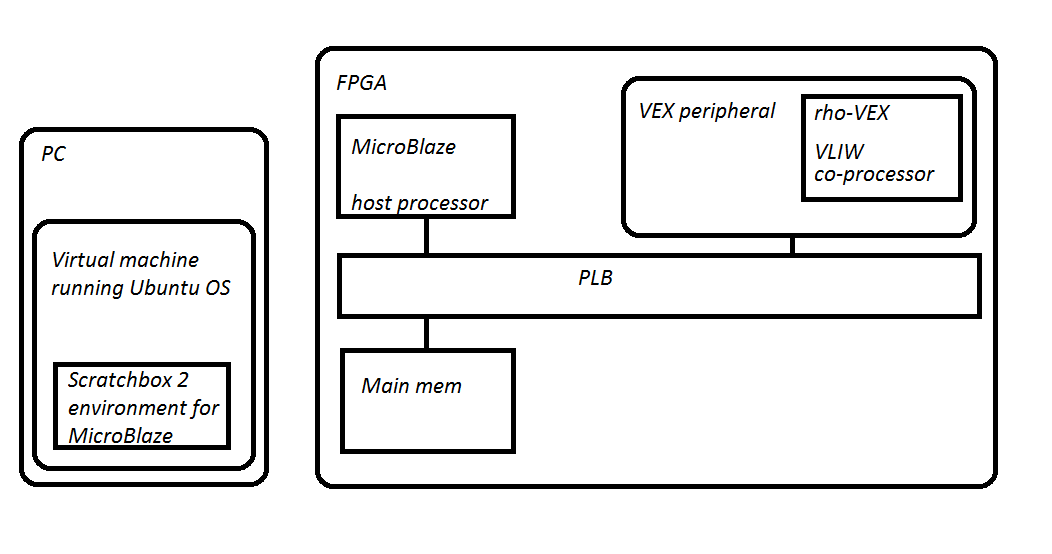
\includegraphics[width=\columnwidth]{Pictures/Platform_paint}%
\caption{Block diagram of the Virtual Machine and the ERA platform}%
\label{lelijk}%
\end{figure}

En nu ga ik lunchen.